\documentclass[10pt]{article}
\usepackage[margin=0.72in]{geometry}
\usepackage{graphicx}
\usepackage{booktabs}
\usepackage{amsmath}
\usepackage{enumitem}
\usepackage{hyperref}
\usepackage{float}
\setlength{\parskip}{0.35em}
\setlength{\parindent}{0pt}

\title{\textbf{Big Data Cup 2026 (Rough Draft v1)}\\Forechecking Pressure Topology}
\author{Working Draft}
\date{February 2026}

\begin{document}
\maketitle
\vspace{-1.1em}

\textbf{Question.} Can we model forechecking as a continuous pressure field (rather than a fixed system label) and use that geometry to predict whether the opponent exits cleanly, is forced to dump out, or turns the puck over?

\textbf{Data + scope.} 10 games from the public BDC 2026 release, 5v5 only. Rule-based segmentation yields 2{,}086 forecheck episodes and 14{,}921 sampled tracking frames (frame stride = 20).

\section*{1. Approach Summary}
For each episode, we identify the puck carrier each sampled frame and compute an ETA-weighted kernel pressure field from forecheckers:
\[
P(x)=\sum_i \exp\left(-\frac{\|x-x_i\|^2}{2\sigma^2}\right)\exp\left(-\frac{\text{ETA}_i(x)}{\tau}\right).
\]
We then extract:
\begin{itemize}[leftmargin=1.2em,itemsep=0.2em]
    \item \textit{Local pressure:} mean/peak pressure at carrier, defender proximity, overlap.
    \item \textit{Topology:} integrated corridor costs (middle, strong boards, weak boards, behind net), most-open corridor cost, and 3s corridor closure rate.
    \item \textit{Shape and squeeze:} pressure compactness area and funnel-to-boards signal (pressure gradient orientation).
\end{itemize}
Episode-level signatures are clustered (k-means, $k=4$) and tested in outcome models (logistic + gradient boosting) against distance/count baselines.

\begin{figure}[H]
    \centering
    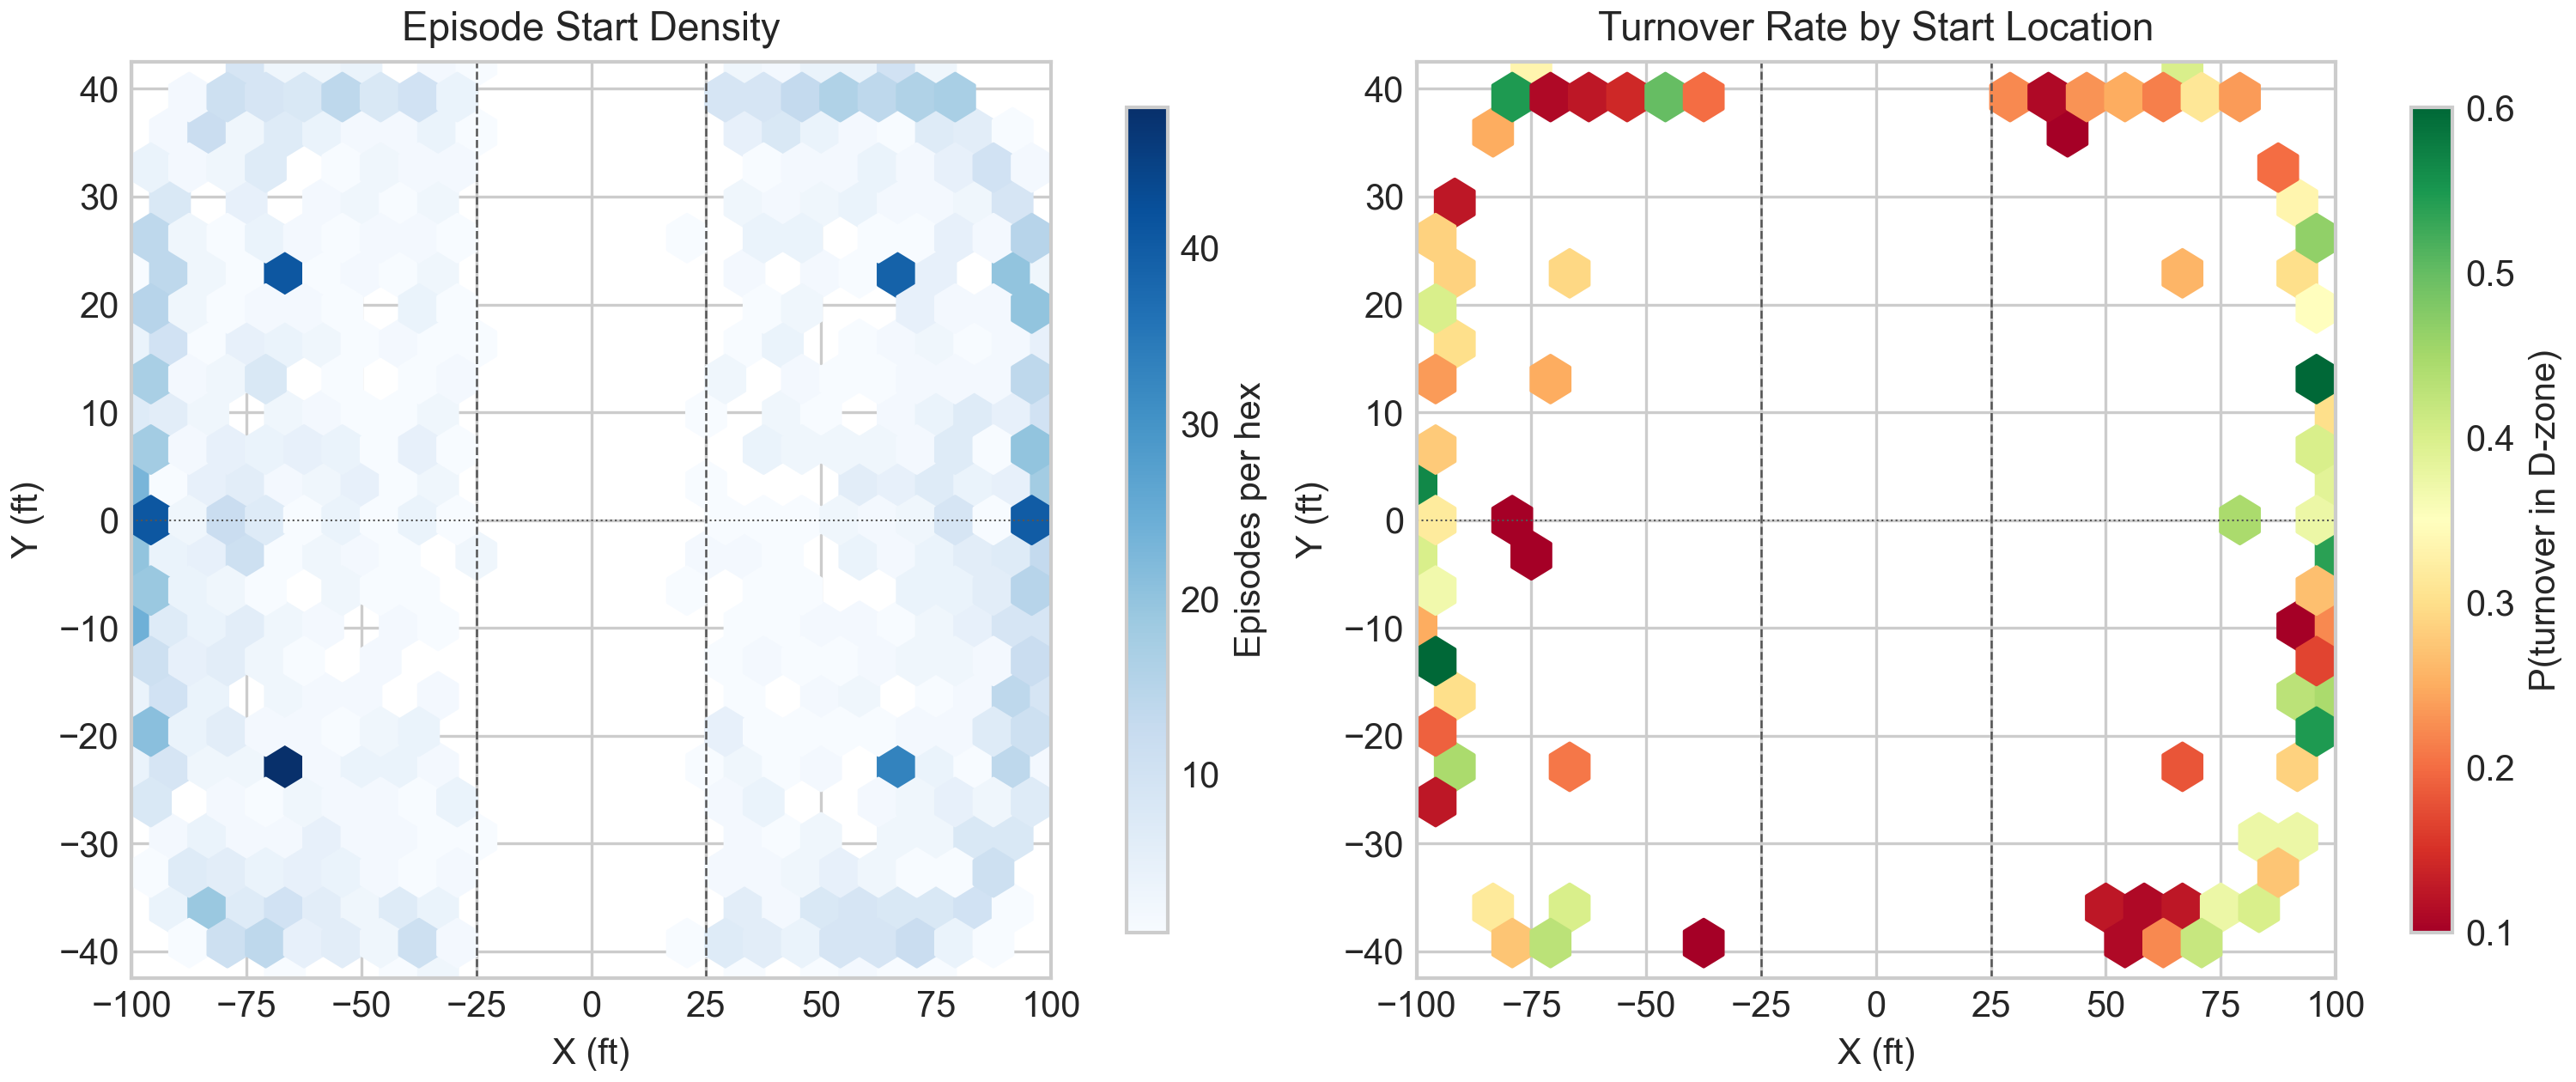
\includegraphics[width=\textwidth]{figures/fig_start_maps.png}
    \caption{Where forecheck episodes begin, and where they are most likely to become D-zone turnovers. High-risk turnover pockets appear in deep corners/half-wall retrieval zones.}
    \label{fig:start_maps}
\end{figure}

\section*{2. Core Findings}
\textbf{Outcome mix.} Across episodes: controlled exits allowed 39.9\%, forced dump-outs 28.6\%, D-zone turnovers 26.1\%.

\textbf{Pressure intensity matters.} In the top pressure quartile, denial events (turnover + forced dump-out) occur on 62.4\% of episodes versus 46.8\% outside that quartile.

\textbf{Topology improves prediction.} Pressure features outperform simple baselines for turnover prediction:
\begin{itemize}[leftmargin=1.2em,itemsep=0.2em]
    \item Gradient boosting with pressure topology: AUC $=0.758\pm0.019$.
    \item Nearest-defender baseline: AUC $=0.640\pm0.025$.
    \item Defender-count baseline: AUC $=0.619\pm0.031$.
\end{itemize}

\textbf{Archetypes are not classic labels.} Cluster C0 is the ``tight-net squeeze'' archetype: high sustained pressure, high compactness, and the best denial profile (33.2\% turnovers, 32.0\% forced dump-outs, 29.9\% controlled exits allowed).

\begin{figure}[H]
    \centering
    \begin{minipage}[t]{0.49\textwidth}
        \centering
        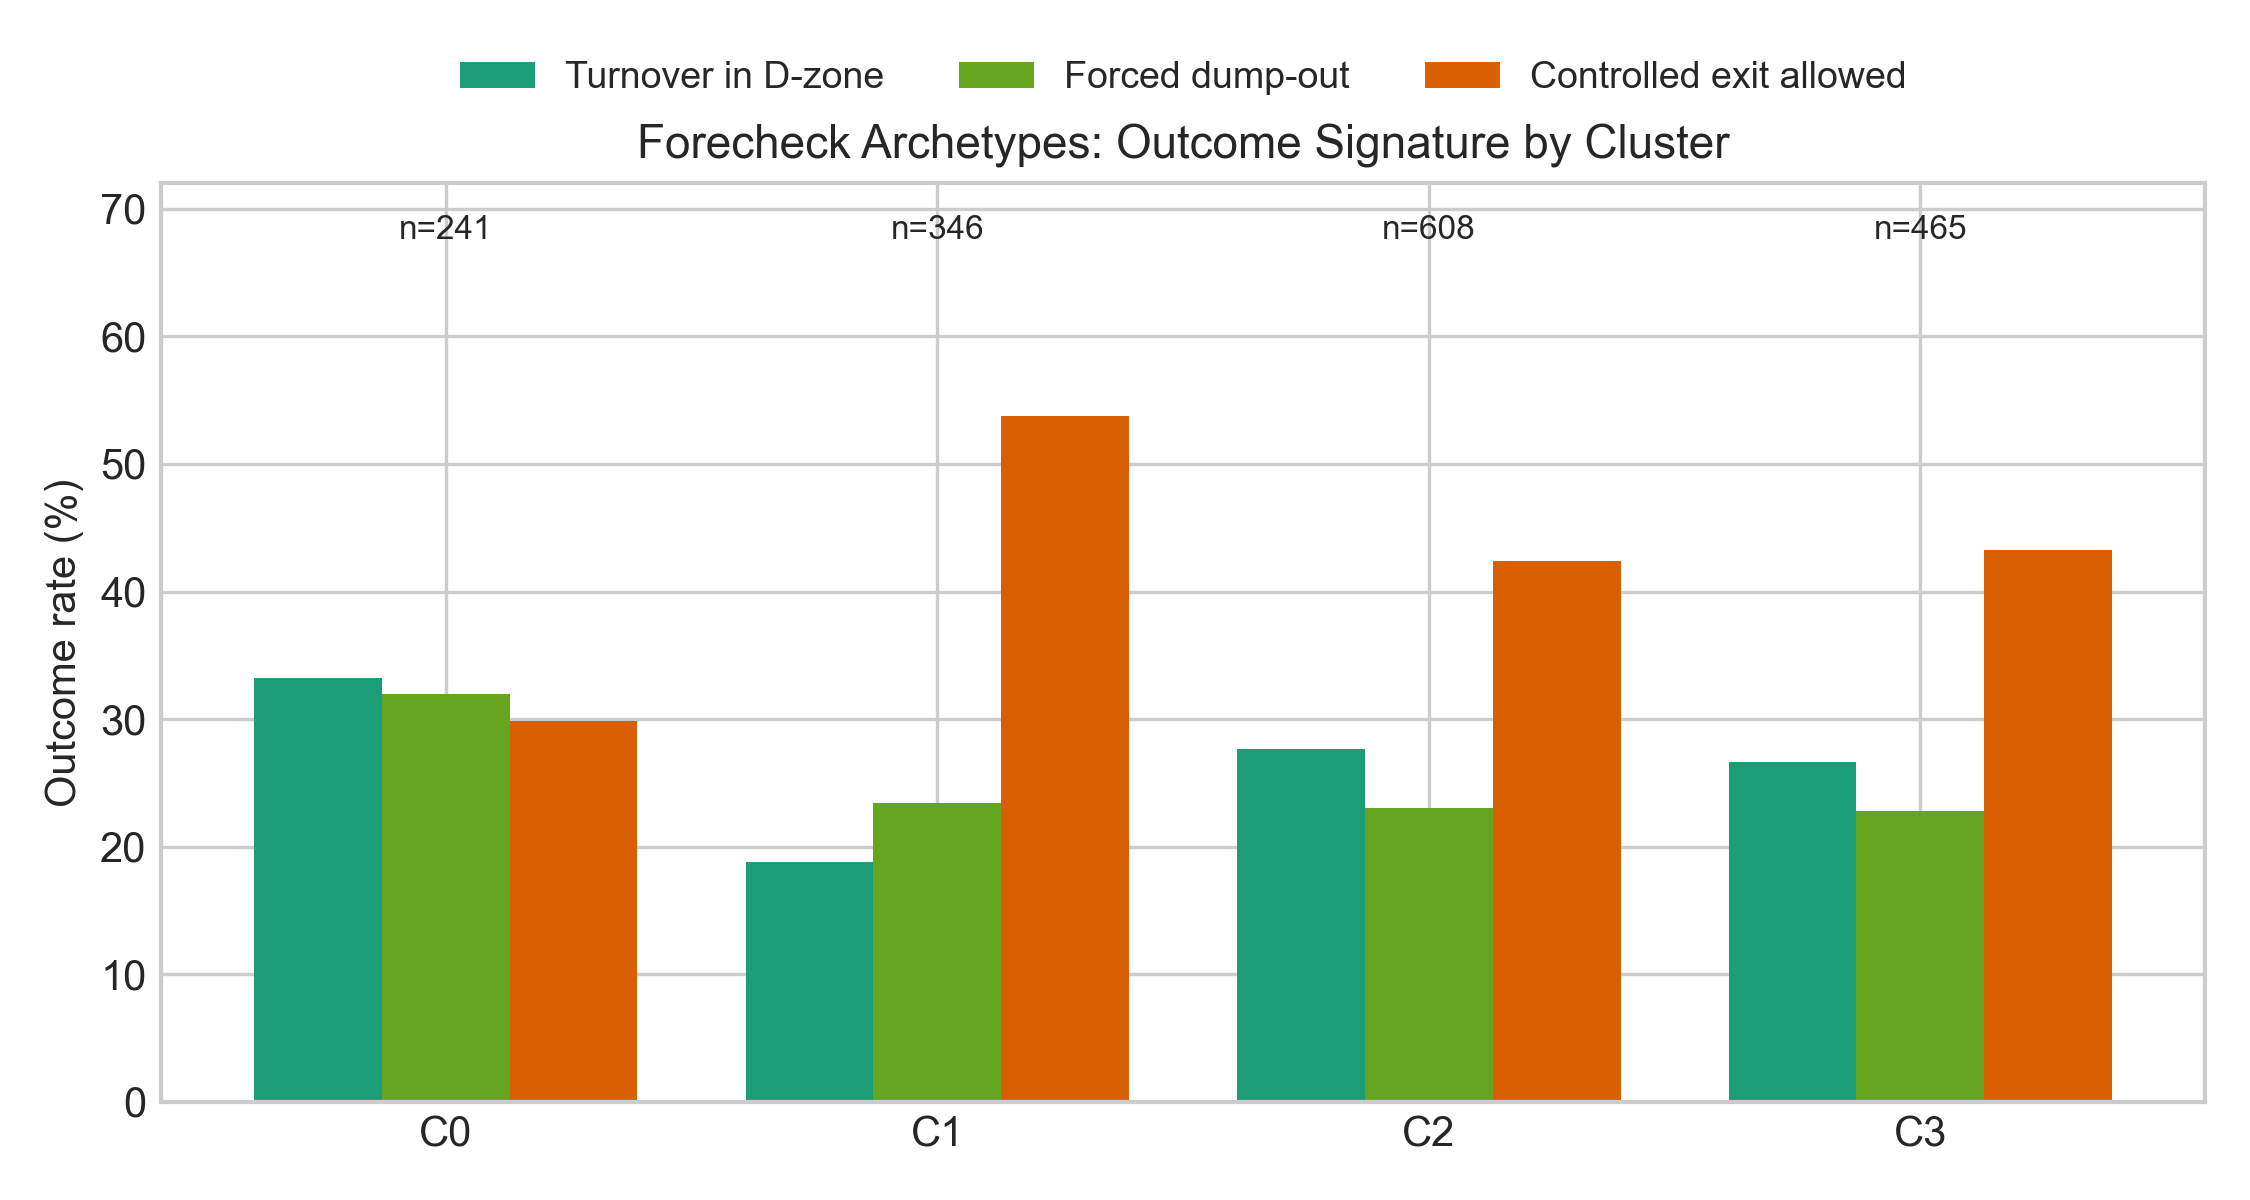
\includegraphics[width=\textwidth]{figures/fig_cluster_outcomes.png}
    \end{minipage}
    \hfill
    \begin{minipage}[t]{0.49\textwidth}
        \centering
        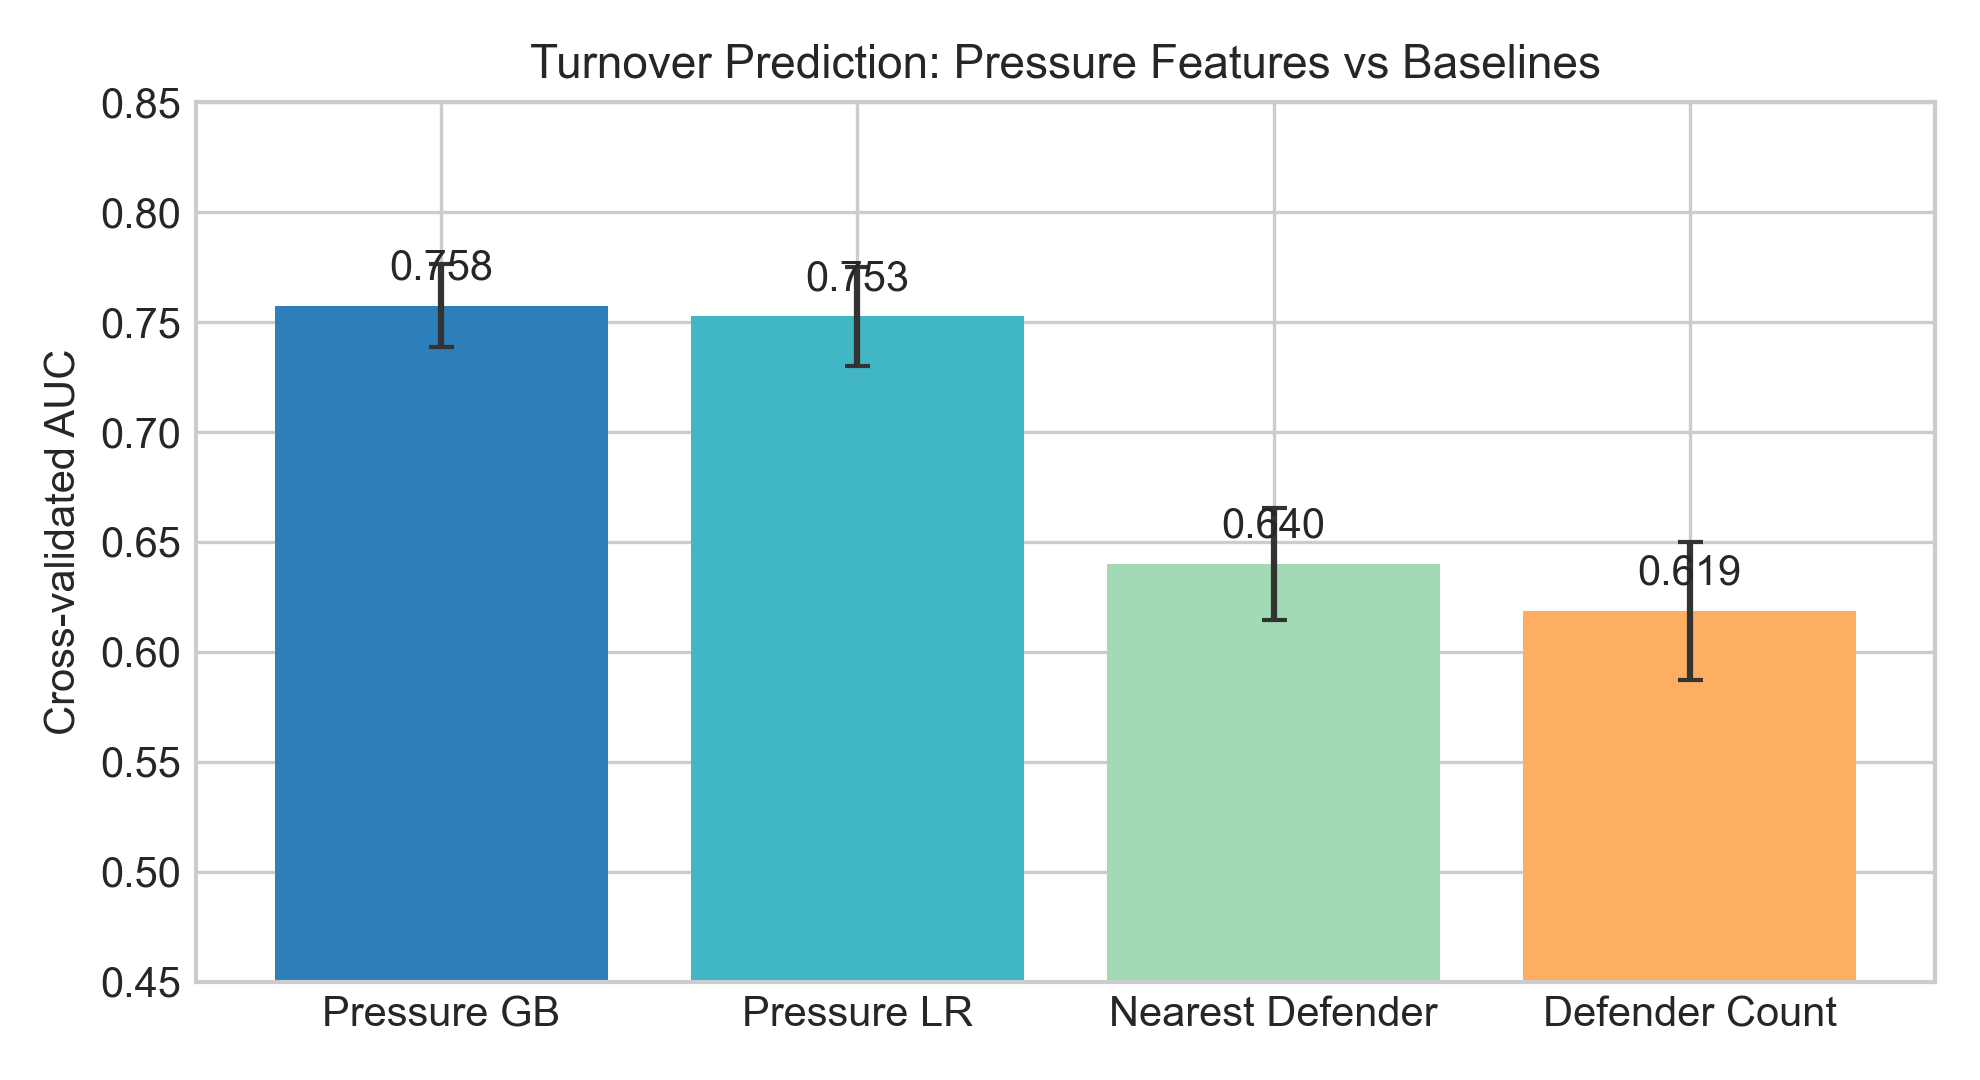
\includegraphics[width=\textwidth]{figures/fig_model_auc.png}
    \end{minipage}
    \caption{Left: outcome signature by pressure archetype cluster. Right: predictive lift from pressure topology versus simple forecheck proxies.}
    \label{fig:cluster_model}
\end{figure}

\section*{3. Actionable Recommendations (GM / Head Coach)}
\textbf{A. Build game-plan around pressure \emph{shape}, not just pressure \emph{count}.}
Drives that simultaneously (i) raise carrier pressure and (ii) collapse open corridors quickly are most disruptive. Practice objective: faster first-3s corridor closure after retrieval.

\textbf{B. Prioritize retrieval-zone ambushes.}
Turnover probability is highest when possession begins deep and near boards; use pre-scout triggers for immediate support layers in those sectors.

\textbf{C. Track team-level TFPI as a process KPI.}
Define \textit{Team Forecheck Pressure Index}:
\[
\text{TFPI}=100\cdot\left(\text{TurnoverRate}+0.5\cdot\text{ForcedDumpRate}-\text{ControlledExitRate}\right).
\]
In this sample, Team I (11.6) and Team L (9.8) lead; Team K (-6.3) and Team B (-4.4) trail.

\textbf{D. Personnel deployment.}
Deploy forward lines/defense pairs that consistently produce C0/C3-like signatures in one-goal or protect-lead situations.

\begin{figure}[H]
    \centering
    \begin{minipage}[t]{0.49\textwidth}
        \centering
        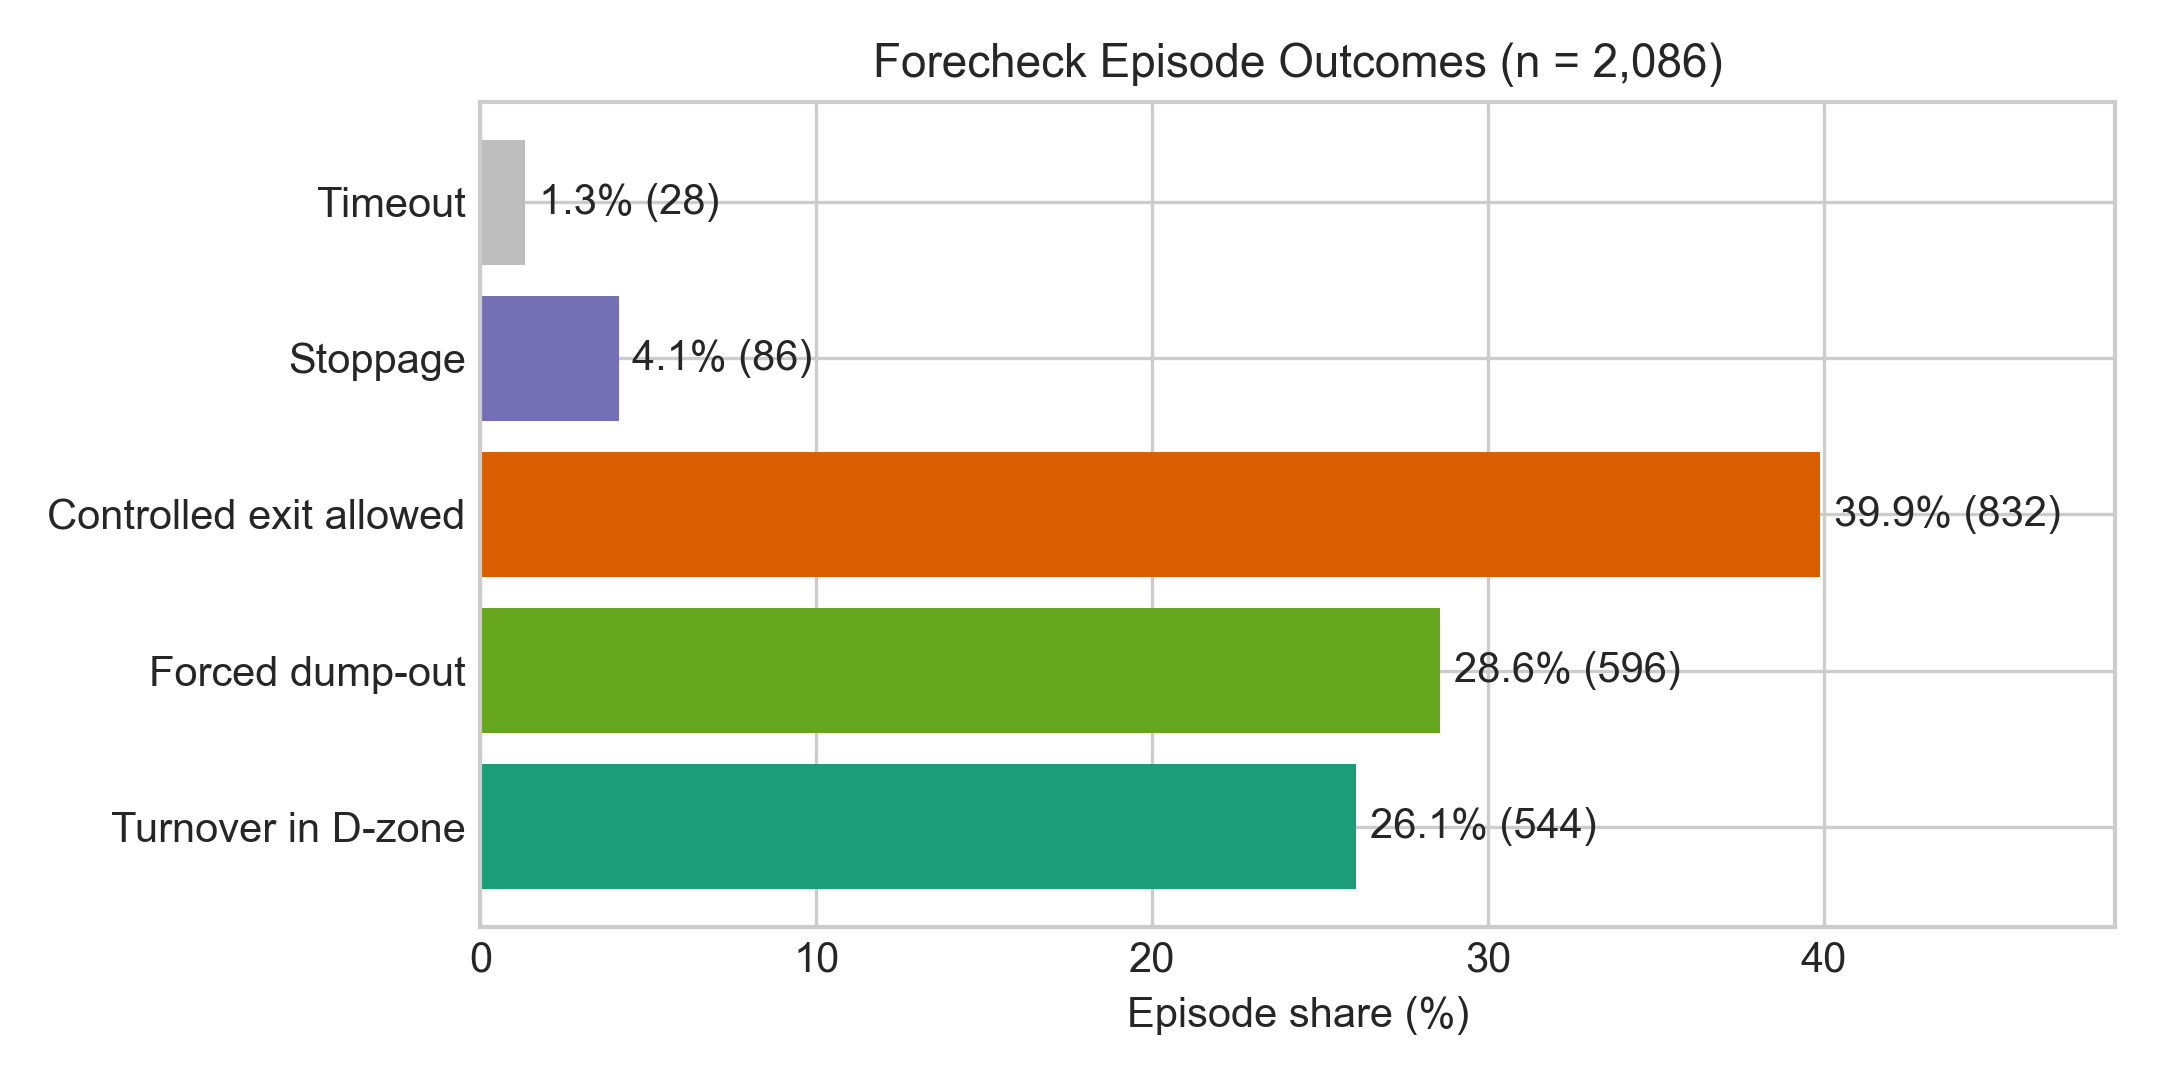
\includegraphics[width=\textwidth]{figures/fig_outcome_distribution.png}
    \end{minipage}
    \hfill
    \begin{minipage}[t]{0.49\textwidth}
        \centering
        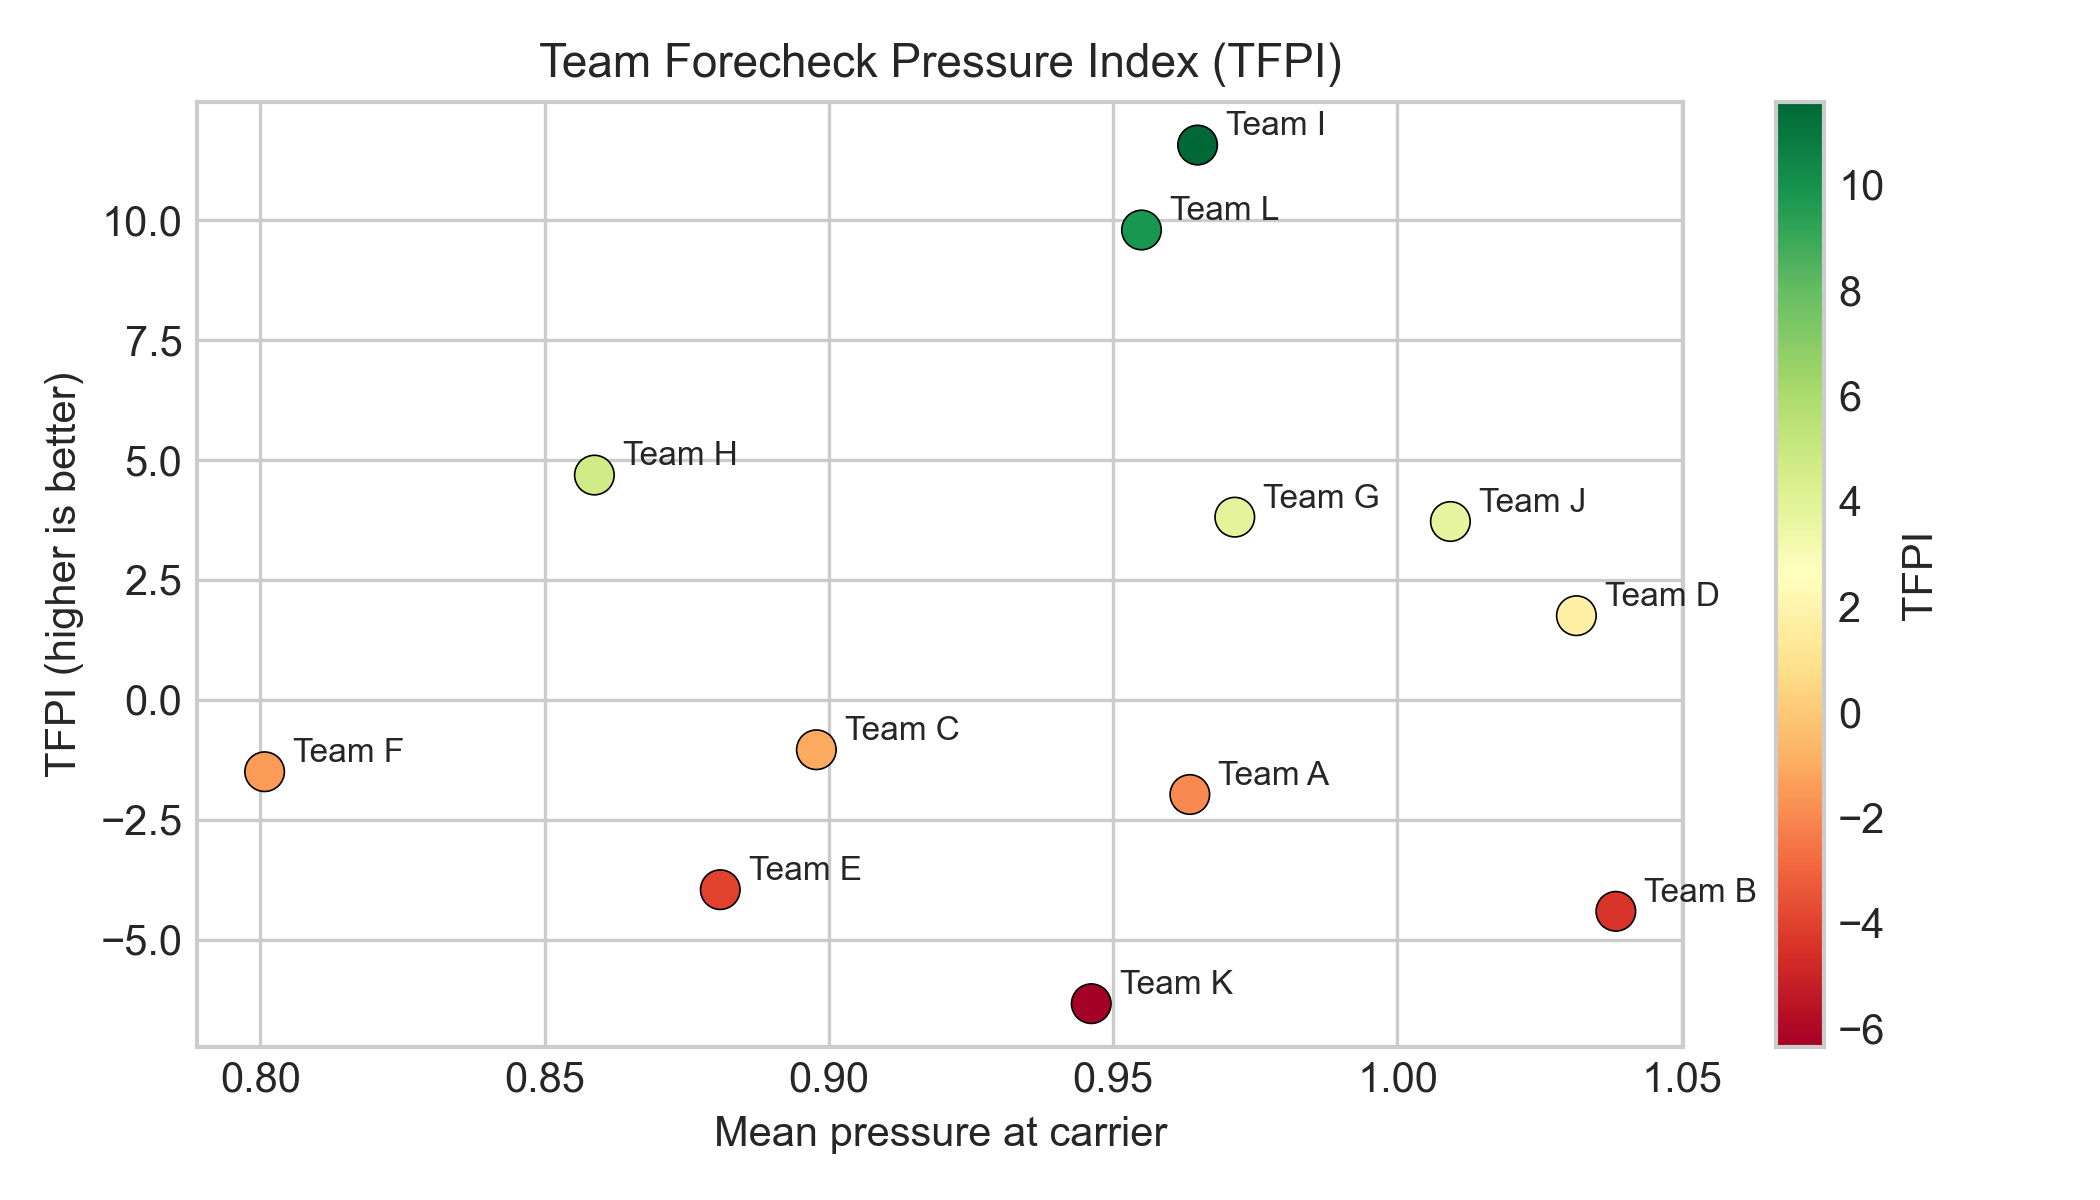
\includegraphics[width=\textwidth]{figures/fig_team_tfpi.png}
    \end{minipage}
    \caption{Episode outcome mix (left) and team-level TFPI benchmark (right).}
    \label{fig:tfpi}
\end{figure}

\section*{4. Limitations and Next Steps}
\begin{itemize}[leftmargin=1.2em,itemsep=0.2em]
    \item Current pressure model is interpretable but not yet acceleration-constrained anisotropic reachability.
    \item Episode segmentation is rule-based; edge-case validation against video should be added.
    \item Next revision: infer F1/F2/F3 roles and estimate player-level Pressure Contribution by role.
\end{itemize}

\textbf{Code + data appendix path:} \texttt{projects/forechecking\_pressure\_topology/}

\end{document}

